\chapter{Kernel-Based Nonlinear Spatial Transformation}\label{ch:spheremapping}
\section{Introduction}

As proposed in last chapter, the objective of the proposed system is to predict subsequent abnormalities by quantifying the deviation of a sample. Whereas the original cluster geometry in feature space $\Omega^d$ depends on the feature extraction stage $g()$. With the extracted features, the cluster geometry may not present a necessary symmetric property and will thus lead to poor performance or even failure in predicting subsequent abnormalities. 
Therefore, an optimization using spatial transformation is addressed to solve this problem. More specifically, the designed method is able to maximize angles between vectors of normal cluster centroid to each abnormal cluster center centroids. In this chapter, a kernel-based nonlinear spatial transformation is proposed to reshape the feature space to reach the required symmetric property. The geometry of reshaped feature space should possess the following features:
 \begin{itemize}
     %\item Vectors pointing from normal centroid to different abnormal clusters centroids has no overlapping or cross with each other.
     \item Vectors pointing from normal centroid to different abnormal clusters centroids have maximum mutual cosine distance.
     \item The overlapping part of all clusters is minimized.
 \end{itemize}

%However the geometric structure of clusters in the feature space $\Omega$ depends on the feature extraction stage $\g()$. The geometric structure of extracted feature in Table.\ref{table:features} does not meet the standards mentioned above.
Given that clusters in original feature space do not meet the symmetric property mentioned above and a spatial transformation is required, we assume in this chapter that new feature space obtained by non-linear reshaping is noted as $\Phi^{d'}$. This reshaping process is included in the Personal Classifier stage (as shown in Fig.\ref{fig:flow}) of the ECG classification system as described in chapter 2. The nonlinear mapping projects each sample $\mathbf{x}_k$  onto a new vector $\mathbf{z}_k$ in a higher dimensional space, which can be considered as the union of subspaces for each type: $\Phi^{d'}=\{\mathcal{N},\mathcal{S},\mathcal{V},\mathcal{F}\}$, where $d'>d$


\section{Kernel Method}

Kernel method has been widely applied in the machine learning algorithms, among which nonlinear Support Vector Machine (SVM) has been utilized in numerous applications recently\cite{shawe2004kernel}. Nonlinear kernel method can efficiently improve classification performance when there exists a nonlinear relationship between input and output variables. Because of the complexity and variety of feature vectors used in ECG analysis, the nonlinear relationship assumption is considered valid in this work. Therefore, it is practical to incorporate the nonlinear kernel method in the ECG analysis system.

In kernel SVM, the nonlinearities are introduced to the model by a kernel, which implicitly maps data $\mathbf{x}$ in input space $\Omega$ into a Hilbert space $\Phi$ via a function $\Psi()$\cite{aronszajn1950theory}. And the algorithm  minimize the expected error $E[L(y,f(x)]$ so as to obtain the final classification mapping function $f$ defined by $\Psi()$, where $L$ is the designated loss function, such as square error $(y-f(x))^2$ \cite{scholkopf1999advances}. If there are $m$ observations in the input space, we use notation $\mathbb{N}$ for index set ${1:m}$. Based on the input space $\mathbf{x_i}\in \Omega (i\in \mathbb{N})$ and classification mapping function $f$, the optimization problem can be written as:

\begin{align}
    \text{minimize}~\frac{1}{m}\sum_{i\in \mathbb{N}}L(y_i,f(\mathbf{x_i})) + \gamma||f||^2
    \label{eq:kernel}
\end{align}

where, $||f||^2$ is the squared norm of $f$% on Hilbert space $H_K$. 
; positive constant $\gamma$, also known as the regularization parameter, controls the balance between training error and the model complexity (smoothness).
%For example, if $H_K$ is the Hilbert space of linear functions, the $f$ can be written as $f=w' x,~w\in\mathbb{R}^d$. Therefore, the loss function can be written as:

%\begin{align}
%    \frac{1}{m}\sum_{i\in \mathbb{N}}L(y_i,w'\mathbf{x_i}) + \gamma w'w
%    \label{eq:kernel}
%\end{align}

%Positive constant $\gamma$, also known as the regularization parameter, controls the balance between training error and the model complexity (smoothness). 
When optimizing the objective function above, SVM only requires the inner products of the mapped features $\Psi(\mathbf{x})$ in Hilbert Space $\Phi$. Therefore, a kernel defined as $k(\mathbf{x_i},\mathbf{x_j}) = \Psi(\mathbf{x_i})^T\Psi(\mathbf{x_j})$ can efficiently substitute inner product calculation and introduce necessary nonlinearities in the model\cite{evgeniou2000regularization}.

%In SVM and other machine learning models, nonlinear kernel methods are implemented with different loss functions \cite{evgeniou2000regularization}. But in more general conditions, the solution to Eq.\ref{eq:kernel} can be written as follows: 

%\begin{align}
%    f(x)=\sum_{i\in \mathbb{N}}c_i K(\mathbf{x_i},\mathbf{x} )
%    \label{eq:kernel2}
%\end{align}

%where ${c_i: i \in \mathbb{N}}$ is a set of real number, $K$ is a kernel such as a polynomial kernel of order $r$: $K(x,t)=(x't)^r,~x,t\in \mathbb{R}^d$.

%For any kernel $K$, it has the following properties: i) for $\mathbf{x} \in \Omega$, $K(\mathbf{x},\cdot)\in H_K$; ii) for $f\in H_K$, $<f,K(\mathbf{x},\cdot)>_K = f(\mathbf{x})$, where $<\cdot,\cdot>_K$ represents the inner product of $H_K$\cite{aronszajn1950theory}.

%A kernel is usually defined base on feature mapping concept, in this work we define this mapping function as $\Psi:\Omega^d\to \Phi^{d'}$ %where $\Psi^{d'}$ is Hilbert space and $<,>_{\Phi}$  represents inner product. 
%Therefore, Eq.\ref{eq:kernel2} can be also written as:

%\begin{align}
%    f(x) = \sum_{i\in \mathbb{N}}c_i \Psi(x_i,x)
%\end{align}



Different kernels represent distinctive nonlinear mapping functions. For machine learning models, the selection of kernel plays a decisive role. An effective kernel function generally needs to satisfy Mercer theorem \cite{cristianini2000introduction}. 
%This means the matrix defined by function $\Psi(x_j,x)$ is symmetric positive semi-definite. In general, the selection of kernel function depends on all observations in input space. 
Whereas, exhaustively searching for all possible kernel is computationally expensive and unrealistic\cite{chapelle1999support}. A more efficient way to resolve this problem is to search for the optimal weighted combination of a set of base kernels, such as polynomial kernel function and Gaussian kernel function\cite{lanckriet2002robust}. This method has been proven to be robust and efficient since the base kernels satisfy Mercer’s condition individually and is consistent with different dataset\cite{jebara2004multi}.
%However, in effect, kernel functions with simple expression, such as polynomial kernel function, Gaussian kernel function and exponential kernel function are usually preferred than complicated kernel function for its simplicity and consistency. 

Polynomial kernel is usually applied on normalized data for its explicit expression and steady performance. Whereas the degree of freedom of polynomial kernel is comparatively high, which leads to a large number of parameters. Gaussian kernel function, a very classic robust radial function, has high robustness when strong noise presents in the dataset. Nevertheless, since Gaussian kernel actually projects samples to an infinite dimensional space, it's difficult to visualize the projected observations $\Psi(\mathbf{x})$ and interpret the result. %Moreover its performance is greatly affected by parameter selection.

In this work, the representative polynomial kernel is selected for the purpose of validating the proposed method and interpreting the effect of optimized nonlinear kernel method on feature space reshaping. The mapping functions, which is a weighted combination of polynomial kernel can be explicitly written in the following format:

\begin{align}
\mathbf{z}_k
=\mathbf{\Psi_{w}} (\mathbf{x}_k) = 
\begin{bmatrix}
w_{1}  \\
w_{2}   \\
\vdots \\
w_{d^\prime} 
\end{bmatrix}
\circ
\begin{bmatrix}
\psi_1(\mathbf{x}_k)\\
\psi_2(\mathbf{x}_k)\\
\vdots\\
\psi_{d^\prime}(\mathbf{x}_k)
\end{bmatrix}
\label{eq:z}
\end{align}

where $\mathbf{w}$ is the coefficient of weight. Instead of selecting kernel, %The example above shows that regardless the selection of kernel function, parameter optimization will play a critical role. For instance, in this work, 
the process of spatial geometry optimization is accomplished by adjusting the coefficients of fixed polynomial basis functions $\psi()$. Since the number of parameters to adjust will increase exponentially when the order of polynomial functions increase, exhaustive searching are not practical for parameter optimization. Therefore, it's necessary to implement an heuristic optimization algorithm, in which parameters are obtained by maximizing or minimizing objective functions. More specifically, the nonlinear reshaping module in this chapter aims to adjust mapping coefficient  $\mathbf{w} = [w_1,w_2,\dots w_d]^T$ to achieve the ideal symmetric geometry in the reshaped feature space while maintaining the separation between clusters.


\section{Multiobjective Optimization}

\subsection{Objective Functions}

To illustrate the optimization problem, we assume, in this example, that the original feature space is a 2-dimensional space $\Omega^2$, then the mapping base kernel may adopt second-order polynomial function as follows:

\begin{align}
\nonumber
&\mathbf{x}=[x_1~ x_2]^T,~~ \mathbf{w}=[w_1~ w_2~ \dots~ w_5]^T,~~d=2, ~~d^\prime=5\\
&\psi_1(\mathbf{x})=x_1, \psi_2(\mathbf{x})=x_2, \psi_3(\mathbf{x})=x_1^2, \psi_4(\mathbf{x})=x_2^2, \psi_5(\mathbf{x})=x_1x_2
\label{eq5}
\end{align}

Using similar concept to the loss function in the standard kernel SVM, the following objective functions can be used to represent the symmetric structure to be obtained:

\begin{align}
\label{eq:obj}
&o_1(\mathbf{w}) = \frac{1}{\underset{c,d=2,\dots,p \text{ and } c\neq d }{\min}\{d(\mathbf{v}_{\mathcal{X}_c},\mathbf{v}_{\mathcal{X}_d})\}} \\ %|a,b=1,2\dots k;a\neq b)
\nonumber 
&o_2(\mathbf{w}) = \frac{SW}{SB}=\frac{\sum_{c=1}^{C}  \sum_{\mathbf{z} \in \mathcal{X}_c}   (\mathbf{z}-\mathbf{c}_{\mathcal{X}_c})^T(\mathbf{z}-\mathbf{c}_{\mathcal{X}_c})}{\sum_{c=1}^{C}\sum_{d=1, d\neq c}^{C}  (\mathbf{c}_{\mathcal{X}_c}-\mathbf{c}_{\mathcal{X}_d})^T(\mathbf{c}_{\mathcal{X}_c}-\mathbf{c}_{\mathcal{X}_d}) }
\end{align}

The maximization of pairwise cosine distance between vectors $\mathbf{v}_{\mathcal{X}_{c,d}}$, which connect the centroid of the normal cluster to centroids of abnormal clusters $\mathcal{X}_c$, can be obtained by minimizing $o_1(\mathbf{w})$. In fact, this objective functions is deduced from discrimination function of personal classifier in Eq.\ref{eq:personal_discrim}. Cosine distance is defined by Eq.\ref{eq:cosine} and the calculation of $\mathbf{v}_{\mathcal{X}_{c,d}}$ is as follows: %In the formula, vectors used to measure symmetry is defined by abnormal sample sets in training set DS1 and the personal normal cluster as follows:

\begin{align}
\mathbf{v}_{\mathcal{X}_i} = \mathbf{c}^k_N -  \mathbf{c}_{\mathcal{X}_i}
\end{align}

Since, for some patients, the total number of a certain type of abnormal samples are very limited, abnormal samples in trainign set DS1 are utilized in calculating the two objective functions. In Eq.\ref{eq:obj}, the abnormal cluster centroids are calculated using abnormal sample sets in training set DS1, while the normal cluster centroid is defined by the personal normal cluster. 

On the other hand, $o_2(\mathbf{w})$ represents the ratio of within-cluster variance to between-cluster variance and consequently controls the separation between clusters. By minimizing $o_1(\mathbf{w})$ and $o_2(\mathbf{w})$ jointly, the algorithm eliminates the ambiguity while using Eq.\ref{eq:personal_discrim} to discriminate latent abnormal state and improves the predictive capability.

\subsection{Multiobjective Particle Swarm Optimization}

We noticed that $o_1(\mathbf{w}) $ and $o_2(\mathbf{w})$ are not necessarily independent to each other. Thus, the optimization problem defined above is equivalent to joint minimization of $o_1(\mathbf{w}) $ and $o_2(\mathbf{w})$ subject to a constraint condition: $|w|_2=1$. Since this is a non-convex multiobjective optimization problem, closed form solution as well as the optimization methods for convex function are not adopted in this method. In this work, we utilize Multiobjective Particle Swarm Optimization (MOPSO) algorithm to solve this optimization problem and obtain the optimal coefficients.

Particle Swarm Optimization (PSO) has the advantage of fast-converging, heuristic searching and easy implementation\cite{coello2002mopso, alvarez2005mopso}. Therefore, researchers have been investigating in extending PSO to multiobjective optimization problems. In the framework of MOPSO, the goal is to solve the typical Pareto optimization problem based on the algorithm in PSO. In other words, it aims at solving an optimization problem with two or more conflicting objective functions by approximating the Pareto front. 

\subsubsection{Pareto Front}

In order to compare different set of coefficient in this opmization problem, the concept of Pareto front is briefly introduced in this section. For a multiobjective optimization problem with two objective function, if a solution $\mathbf{w}^1$ is said to \textit{dominate} another $\mathbf{w}^2$ when the following two conditions are satisfied:
\begin{enumerate}
    \item $o_1(\mathbf{w}^1) \leq  o_1(\mathbf{w}^2)$ and $o_2(\mathbf{w}^1) \leq  o_2(\mathbf{w}^2)$ 
    \item $o_1(\mathbf{w}^1) <  o_1(\mathbf{w}^2)$ or $o_2(\mathbf{w}^1) < o_2(\mathbf{w}^2)$ 
\end{enumerate}

If a solution is not dominated by any other solutions in the searching space, then this solution is an \textit{optimal} solution for this problem. A Pareto front is defined by the set of Pareto optimal solutions. However, in non-convex optimization, the Pareto front can not be represented explicitly by a deterministic function. Therefore, the majority of algorithms use heuristic searching algorithms to approximate the Pareto front\cite{coello2002mopso}.

\subsubsection{MOPSO}

Among all the MOPSO algorithms in the literature, the algorithm proposed by Coello Coello and Lechug presents a better performance and lower computational complexity than most of the other MOPSO algortihms\cite{coello2002mopso}. Therefore, this algorithm implemented to solve the optimization problem in this work. One characteristic property of this algorithm is the external repository, in which all Pareto optimal particles for every swarm is recorded for each iteration. The solution represented by repository members are stored and used as an optimal approximation of the Pareto front because they converge to the actual Pareto front as proved in \cite{coello2002mopso}. Fig.\ref{fig:repo_members}, which is generated by jointly minimizing $o_1(\mathbf{w}) $ and $o_2(\mathbf{w})$, demonstrates the repository members are Pareto optimal than other particles and they converge to a uniform Pareto front.

\begin{figure}[t]
\centering
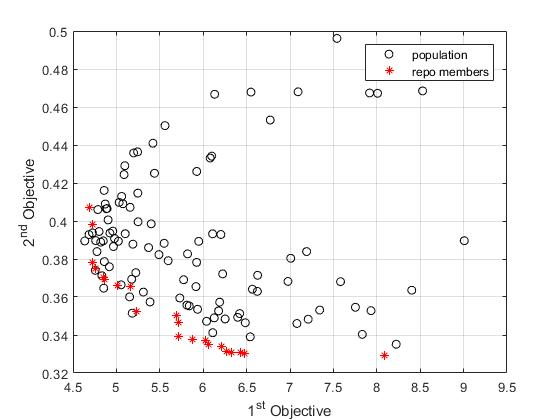
\includegraphics[scale=.6]{Fig/repo_members.jpg}
\caption{Particles stored in external repository approximate the Pareto front}
\label{fig:repo_members}
\end{figure}

With the concept of Pareto optimal, we further demonstrate the impact of applying kernel functions in this spatial reshaping problem by comparing the optimal solutions for coefficients of linear function combination and those for coefficients of polynomial kernel functions. Therefore, we first optimize the coefficients of third-order polynomial kernel functions, as formulated in Eq.\ref{eq5} and then optimize coefficients of linear features in origin feature space. The purpose is to verify if the objective functions can be fundamentally better optimized by introducing nonlinearities into the model. %A two-dimension curve formed by repository members t will be drawn with two objective functions.

%This mapping by kernel method can be accounted as the input space reshaping, namely, new input sample space is produced using non-linear kernel bending feature space in order for a higher space symmetry. Reshaping result as indicated in diagram 4-6 can be obtained through testing the reshaping algorithm with test data and quadratic polynomial. More specifically, we can regard this kernel method as a mapping from two-dimension space   to three-dimension space. Because the data visualization is very important in the test, we don’t adopt polynomial kernel of higher degree.

As shown in Fig. \ref{fig:pareto_compare}, the estimated Pareto front of the nonlinear model using polynomial kernel obviously dominates the Pareto front of linear model consist. The result shows that optimization with nonlinear kernel functions possess a higher degree of freedom and is able to find optimal solutions than the best solutions by linear combination. In other words, kernel method combined with multiobjective particle swarm optimization algorithm can improve the spatial structure of clusters according to the two objective functions.

%\subsubsection{Pareto Front}
\begin{figure}[t]
\centering
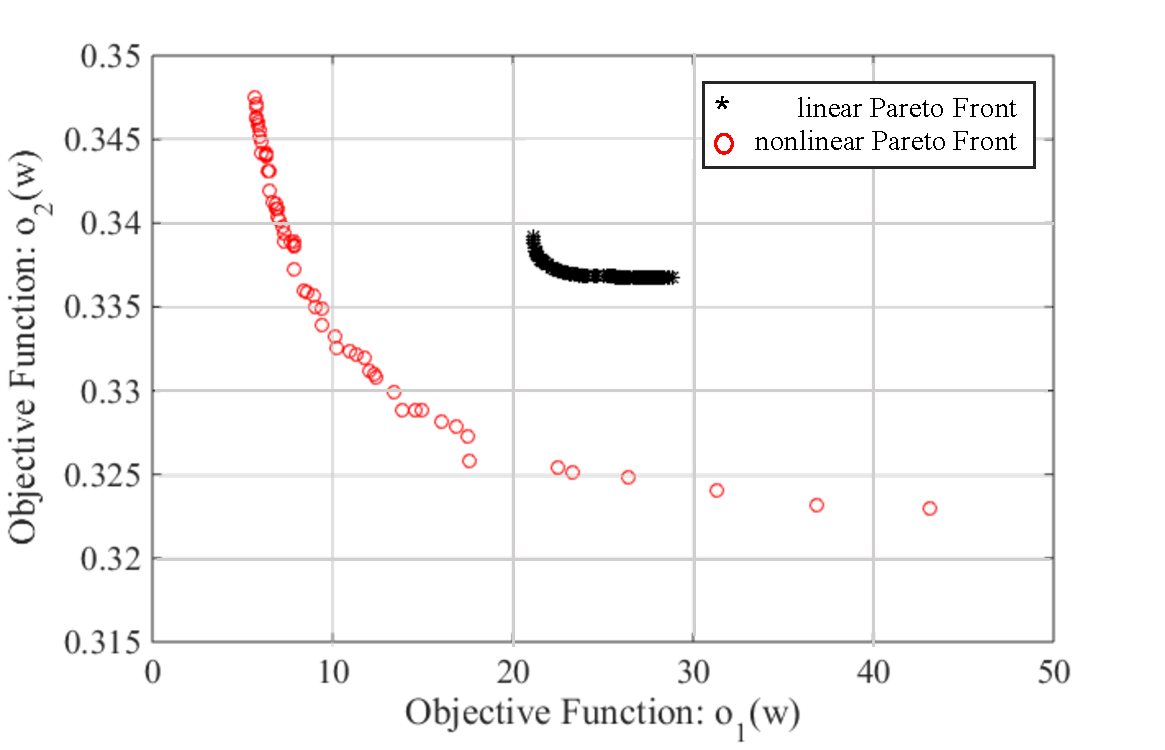
\includegraphics[scale=.6]{Fig/pareto_compare.pdf}
\caption{Increase of degree of freedom in optimization is proved by comparing the Pareto fronts generated by linear and nonlinear basis function}
\label{fig:pareto_compare}
\end{figure}

\section{Experimental Results}\label{sec:result1}

%This section will introduce the experimental result of the aforementioned kernel-based method on test set DS2 of MITDB to show the performance. 
As mentioned in Section. 2.3, a cardiac segment is represented by an 8-dimensional vectors after feature extraction and PCA. %In order to reduce the complexity,  we firstly map the original 22-dimensional feature vectors, representing cardiac segments, into an 8-dimensional vectors $\mathbf{x}_{8 \times 1}$ using Principal Component Analysis (PCA). 
To specify the nonlinear transformation in (\ref{eq:z}), the polynomial functions of order $3$ is applied on the feature vectors. Moreover, taking the overfitting problem in high-dimensional space and computational cost into account, only $32$ terms, which include 8 square terms $x_i^2$, 8 cubic terms $x_i^3$, 8 cross terms $x_ix_j$ of second order and 8 cross terms $x_i x_j^2$ of third order, are retained by randomly discard the redundant cross terms. Therefore, the mapped vectors $\mathbf{z}_{32 \times 1}$ include a total of $32$ terms as follows.

\begin{align}
\label{eq:8-32}
\mathbf{z}&=\{x_i^2|i=1,2\dots 8\}\cup\{x_i^3|i=1,2\dots 8\} \cup\\
\nonumber
& \{x_ix_j|i,j=1,2\dots 8,i\neq j\} \cup  \{  x_i^2x_j | i,j=1,2\dots 8,i\neq j \}
\end{align}

The performance of the aforementioned kernel-based method is tested on DS2 excluding record 232, for this record has only 7 normal samples $y_k=N$. In total, 21 records are tested.

Table \ref{table:result1} shows the performance of the proposed method in classifying ECG signal segments. In order to evaluate the consistency and general classification classification results over all recordings, the median, interquartile range (IQR), mean and standard deviation of accuracy (AC), sensitivity (SE) and specificity (SP) are presented as evaluation metrics. The results are promising and the median of accuracy for all classes are in the range of $88\%-99\%$. Sensitivity and specificity of the proposed method exhibits similar ranges. The mean accuracy is at least $86\%$ excluding class $V$. Therefore, this system is not likely to miss an important alarm or to report false alarms. 

\begin{table}[t]
	\caption{Classification results of the proposed method.}
	\centering
	\begin{tabular}{|c|c|c|c|c|}
		\hline
		Class N & median(\%) & IQR(\%) & mean(\%)& std (\%) \\ 
		\hline 
		AC & 94.8& 19.52 & 86.62 & 18.55\\ 
		\hline 
		SE & 97.21  & 17.36 & 87.47 &19.26 \\ 
		\hline 
		class V & median(\%) & IQR(\%) & mean(\%)& std (\%) \\ 
		\hline 
		AC & 86.11 & 27.54 & 76.41 & 22.81 \\ 
		\hline 
		SP & 99.71 & 11.22 & 90.18 & 18.52 \\ 
		\hline 
		class S & median(\%) & IQR(\%) & mean(\%)& std (\%)\\ 
		\hline 
		AC & 99.28 & 2.24& 98.29&2.57 \\ 
		\hline 
		SP & 99.64& 22.17& 97.56 & 6.06\\ 
		\hline 
		class F & median(\%) & IQR(\%) & mean(\%)& std (\%) \\ 
		\hline 
		AC & 97.91 & 8.2&93.85&7.84\\ 
		\hline 
		SP & 100.00 & 0.03&99.12&3.6\\ 
		\hline 
	\end{tabular} 
	\label{table:result1}
\end{table}

%%%%%%%%%%%%555

More importantly, the predictive capability of the proposed method is worthy of evaluating exclusively for it is the featuring specialty of the proposed system. In order to quantify the posterior probability of observing an abnormal signal after a preceding yellow alarm of similar type in (\ref{eq:personal_discrim}), the number of predicted samples are counted as formulated in Eq \ref{eq:proab}:

\begin{align}
\nonumber 
&P(\hat{y}_{k+i}=X_r|\hat{y}_{k}=X_y)=\frac{\text{\# of $y_{k+i}=X$ after $\hat{y}_k=X_y$}}{\text{\# of true alarms after $\hat{y}_k=X_y$}} \\
&P(\hat{y}_{k+i}=X_r)=\frac{\text{\# of true alarm of type $X$ ($y_{k}=X$)}}{\text{\# of all true alarms}} 
\label{eq:proab}
\end{align}

The summary of results for all 21 test records is presented in Table. \ref{table:pred}. The subsection \textit{Probability of next abnormality (\%)} in Table. \ref{table:pred} shows the confusion matrix of the probability of having a subsequent true abnormality of all types after observing a yellow alarm of all types along with the prior probability of observing a certain type of abnormal sample in the very last column. %The last 4 columns of the Table. \ref{table:pred} show the confusion matrix of the probability of having a subsequent true abnormality of all types after observing a yellow alarm of all types. It's compared with the probability of having the same type of abnormality after a secondary abnormality of its own type. 

These results validate the predictive capability of yellow alarms. 
For instance, the prior probability of observing a sample segment with abnormal types $V$, $S$, and $F$ is respectively $\frac{96}{96+29+18}=67\%$, $\frac{29}{96+29+18}=20\%$ and $\frac{18}{96+29+18}=13\%$, based on their relative frequencies in the dataset. However, the corresponding posterior probabilities after observing a yellow alarm of type $Vp$ are respectively $\frac{38}{38+11+2}=75\%$, $\frac{11}{38+11+2}=21\%$ and $\frac{2}{38+11+2}=4\%$. This means that the probability of observing a real abnormal segment of type $V$ is $75\%-67\%=8\%$, which is higher than its prior probability. The same trend holds for other yellow alarms as well. The results suggest a more in-depth study of the concept of yellow alarms for heart monitoring. Therefore, we investigate in improving the spatial transformation module of the system and meanwhile reduce the computational cost in Chapter 4.

\begin{table}
	\caption{Predictive power of yellow alarms: A yellow alarm increases the chance of observing a red alarm of the same type.}
	\centering
	%\resizebox{\textwidth}{!}{
	\begin{tabular}{|m{6em}| m{2em}| m{2em}| m{2em} |m{2em}| m{2em}| m{2em}| m{2em}| m{2em}|}
		\hline
		& \multicolumn{3}{p{6em}}{Count numbers of subsequent abnormality}& &\multicolumn{3}{p{6em}}{Probability of subsequent abnormality (\%)}  & \\ 
		\hline 
		secondary abnormalities & $V_y$ & $S_y$ & $F_y$ & Total & $V_y$ & $S_y$ & $F_y$ & Total \\ 
		\hline 
		True V & 38 & 23 & 35& 96 & 75 & 75 & 61 & 67 \\ 
		\hline 
		True S & 11 & 10 & 8 & 29 & 21 & 29 & 14& 20 \\ 
		\hline 
		True F & 2 & 2 & 14 & 18 & 4 & 6 & 25 & 13 \\ 
		%		\hline 
		%		Total & 4 & 20 & 0 & 24 & 100 & 100 & 100 & 100\\
		\hline 
	\end{tabular}%} 
	\label{table:pred}
\end{table}


\section{Conclusions}

This chapter introduces and studies the kernel-based nonlinear transformation using Multiobjective Particle Swarm Optimization (MOPSO) method. Inspired by the concept of kernel method and loss function utilized in SVM, we implement the method with a weighted combination of base nonlinear kernels to reshape the input feature space by mapping it to a high-dimensional space. The coefficients of kernels are optimized according to two conditions, namely, maximum separation between cluster and maximum cosine similarities between abnormal clusters.

Result shows that approximated Pareto front produced by kernel method in the objective function space is apparently optimal to the one which is produced by the linear combinations of original features. The results verify that the proposed method has a classification accuracy in the range of $88\%-99\%$ for different ECG records in the test set of MIT-BIH database.

Above all, the proposed algorithm demonstrates the potential of providing detailed information about the sample deviations, which indicate the upcoming abnormal sample types. The predictive capacities of the system is verified with ECG signal, but this method is general and not bound to this application. If a biomedical signal has one base class (i.e. normal state) and several abnormal states, the proposed method can be implemented to predict upcoming abnormal types.
  